% This file is isea.tex. It contains the formatting instructions for and acts as a template for submissions to ISEA 2022. It is based on the ICCC formats and instructions. It uses the files isea.sty, isea.bst and isea.bib, the first two of which also borrow from AAAI IJCAI formats and instructions.
% Modified from ICCC.tex by B. Bogart

\documentclass[letterpaper]{article}
\usepackage{isea}
\usepackage[pdftex]{graphicx}
\usepackage{times}
\usepackage{helvet}
\usepackage{courier}
\usepackage[numbers]{natbib}
\pdfinfo{
/Title (ISEA2022 Formatting Instructions for Authors)
/Author (ISEA 2022)}
% The file isea.sty is the style file for ISEA 2022 proceedings.
%
\title{ISEA2022 Formatting Instructions for Authors}
\author{1\textsuperscript{st} Author Name, 2\textsuperscript{nd} Author Name,  \ldots, n\textsuperscript{th} Author Name (LEAVE BLANK FOR SUBMISSION) \\
Affiliation(s) (LEAVE BLANK FOR SUBMISSION)\\
Location, Country (LEAVE BLANK FOR SUBMISSION)\\
Contact Emails (LEAVE BLANK FOR SUBMISSION)\\
\newline
\newline
}
\setcounter{secnumdepth}{0}

\begin{document} 
\maketitle
\begin{abstract}
The Proceedings of the International Symposium on Electronic
Art will be compiled from electronic manuscripts submitted by
the authors. This paper provides brief style instructions that will
facilitate high-quality, consistent, proceedings. The title
``Abstract'' should be 10 point, bold type, centered at the
beginning of the left column. The body of the abstract
summarizing the thesis and conclusion of the paper in no more
than 200 words should be 9 point, justified, regular type.
\end{abstract}

\keywords{Keywords}

The title ``Keywords'' should be 10 point, bold type, centered at the beginning of the left column. Using 9 point, justified, regular type, write up to ten keywords that highlight the main areas of your essay’s content. 

\section{Introduction}

Your essay’s heading should be 12 point, bold style, centered. Your body text should be 10 point, justified, single space. The first sentence after the heading begins without a paragraph indent like this paragraph.

The second, and subsequent paragraphs are indented 10 points. Do  not  leave  double-space  between   words  or  paragraphs. This sample shows a 10-point Times New Roman text. Times New  Roman  is  the font to be used throughout the essay.

The ISEA2022 submission must be PDF (Portable Document Format) files formatted for 8-1/2'' x 11'' paper.

\subsection{Word Processing Software}

As detailed below, ISEA has prepared and made available a Microsoft Word template and a \LaTeX{} template for use in formatting your paper. If you are using some other word processing software, please follow the format instructions given below and ensure that your final paper looks as much like this sample as possible.

\subsection{Length of Papers}

A variety of paper lengths will be accepted under different categories. Please note that submission lengths must be all inclusive (including references, biographies and acknowledgements).
\begin{itemize}
\item Full paper submissions can be 5-8 pages in the ISEA2022 template format.
\item Short paper submissions can be 2-4 pages in the ISEA2022 template format.
\item Poster and Demo (as extended abstracts) submissions can be up to 2 pages in the ISEA2022 template format.
\item Panel submissions can be 2-4 pages in the ISEA2022 template format.
\item Artist talk can be up to 2-4 pages in the ISEA2022 template format.
\item Institutional presentation submissions can be up to 2 pages in the ISEA2022 template format.
\item For artistic works, workshops and tutorials please use the other appropriate templates.
\end{itemize}

\section{Style and Format}
Templates that implement these instructions can be retrieved at  {\small \tt http://isea2022.isea-international.org/}

\subsection{Layout}

Print manuscripts two columns to a page, in the manner in which these instructions are printed. The exact dimensions for pages are:
\begin{itemize}
\item left and right margins: 0.75''
\item column width: 3.31''
\item gap between columns: 0.38''
\item top margin—first page: 1.25''
\item top margin—other pages: 0.75''
\item bottom margin: 1.25''
\end{itemize}

\subsection{Format of Electronic Manuscript}

For the production of the electronic manuscript, you must use {\em Adobe's Portable Document Format} (PDF). Additionally, you must specify the American {\em letter} format (corresponding to 8-1/2'' x 11'') when formatting the paper.

\subsection{Blind Review}

All submission in the academic call will be reviewed in a double-blind manner.  Please do not include your affiliation and anonymize the text to keep your identity secret.

\subsection{Title and Author Information}

Center the title on the entire width of the page in a 16-point bold font. Below it, center the author name(s) in a 12-point bold font, and then center the address(es) in a 9-point regular font. Credit to a sponsoring agency can appear in the Acknowledgment Section described below.

\begin{figure}[h]
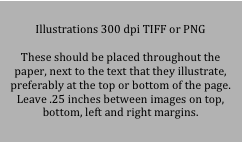
\includegraphics[width=3.31in]{figure.png}
\caption{This is an example of figure caption. Note that all figures, and tables are to be referenced in the text. \copyright Respect Copyright.}
\end{figure}

\subsection{Abstract}

The title ``Abstract'' should be 10 point, bold type, centered at the beginning of the left column. The body of the abstract summarizing the thesis and conclusion of the paper in no more than 200 words should be 9 point, justified, regular type.

\subsection{Text}

The main body of the text immediately follows the abstract. Use 10-point type in {\em Times New Roman} font.

Indent when starting a new paragraph, except after major headings. 

\subsection{Headings and Sections}

When necessary, headings should be used to separate major sections of your paper. (These instructions use many headings to demonstrate their appearance; your paper should have fewer headings.

\subsubsection{Section Headings}

Print section headings centered, in 12-point bold type in the style shown in these instructions. Your body text should be 10 point, justified, single space. Do not number sections.

\subsubsection{Subsection Headings}

Print subsection headings left justified, in 11-point bold type and mixed case (nouns, pronouns, and verbs are capitalized). They should be flush left. Your text should be 10 point, justified, single space. Do not number subsections.

\subsubsection{Subsubsection Headings}

Print subsubsection headings inline in 10-point bold type. Do not number subsubsections.

\subsubsection{Special Sections}

You may include an unnumbered acknowledgments section, including acknowledgments of help from colleagues, financial support, and permission to publish.

The references section is headed ``References,'' printed in the same style as a section heading. A sample list of references is given at the end of these instructions.  Note the various examples for books, proceedings, multiple authors, etc. 

\subsection{Footnotes}

If footnotes are necessary, place them at the bottom of the page in 9-point font. Refer to them with superscript numbers.\footnote{This is how your footnotes should appear.} Separate them from the text by a short horizontal line. 

\subsection{Quotations and Extracts}
Indent long quotations and extracts by 10 points at left margins.

\section{Acknowledgments}
The preparation of these instructions and the \LaTeX{} and Word files was facilitated by borrowing from similar documents used for ICCC proceedings.

\begin{figure*}

\includegraphics[width=\textwidth]{two-column-figure.png}
\caption{Example of a double-column figure with caption. \copyright Respect Copyright.}
\end{figure*}

\section{References}
The title “References” should be 12 point, bold style, centered. Editorial standards adhere to the guidelines set by the Chicago Manual of Style, 16th ed. References should be 9 point, regular type. List them in numerical order immediately after your essay. The numbers should be cross-referenced within the essay, with numbers placed at the end of the sentence in square brackets, with a space after the full stop, as shown at the end of this sentence. \cite{boden92}

\bibliographystyle{isea}
\bibliography{isea}

\section{Author(s) Biography(ies)}
The title ``Author(s) Biography(ies)'' should be 12 point, bold style, centered. Using 9 point, regular type, biographies should be no longer than 150-word count.

\section{Questions?}

For technical questions about Microsoft Word formatting please seek online tutorials. For other questions about your manuscript please contact: {\tt ISEA2022@uoc.edu}


\end{document}
